%every chapter wil be split into a new document. For the sake of the structure, this one_doc strategy is held up
\chapter{Application Area and Goals}
\label{cha:area_goals}
\textcolor{red}{\textit{Do we write a Management summary?}}\\
This paper represents a documentation for the data mining project "Mining the Success for Movies". Information in this paper refers to the (sample) dataset and python scripts handed in for a classification problem. The structure of this paper is as follows: Chapter \ref{cha:area_goals} provides an overview of the problem the project is based on. Goals of the project and the theoretical framework will be discussed as well. Chapter \ref{cha:data_selection} deals with the structure and size of the data. Here, a closer look will be taken at the dataset at hand. Questions that had to be answered were for example which information were provided in the original dataset or which problems were identified concerning for instance outliers or missing values. Chapter \ref{cha:preprocessing_transformation} explains which preprocessing steps had to be taken in order to cleanse the dataset and to prepare it for the data mining step. Chapter \ref{cha:data_mining} describes which data mining techniques regarding algorithms and parameters were used to learn an expedient model in respect of the goals set in Chapter \ref{cha:area_goals}. Chapter \ref{cha:interpretation_evaluation} closes this paper by describing which insights could be won for the problem at hand. Here, a critical reflection is delineated how the model could be improved further in order to provide even more precise results.

\section{Problem Statement}
Already well before new movies are being produced, every stakeholder certainly is interested in the monetary success of the given movie. In order to predict the success costly methods are being applied, such as market investigations. \textcolor{red}{\textit{Do we need a source? koennte noch ausgefuehrt werden.}}

The benefit Data Mining brings to the analysis of large datasets, can also be transferred onto the stated problem of predicting a movie's success. Based on given data of already released movies, a model is being learned which shall be applied on upcoming or planned movies. In order to learn and apply the model various pieces of information are taken into account. Just a few are budget, revenues, runtime, genre and information on the release. Information on the dataset and on all preprocessing methods which were applied will be provided in chapter \ref{cha:data_selection}.

\section{Goals}
The goal of this project is to learn a model which will predict how successful a not yet released movie will be. This is done by using common data mining techniques in Python. As a main objective the question \textit{"Based on revenue, will the movie be popular or will it be a flop?"} shall be answered for all possible combinations of information on a new movie as precisely as possible.
In order to be as precisely as possible, not only different algorithms are being tested, but also parameter tuning is being applied with different performance measures \footnote{Further information on applied techniques and evaluation methods is provided in chapter \ref{cha:data_mining}}.


\begin{itemize}
	\item Problem Statement and idea behind the project
	\item General introduction similar to Project outline
\end{itemize}

\section{Theoretical framework}
\begin{itemize}
	\item keep it small
	\item roughly 1 Page
\end{itemize}
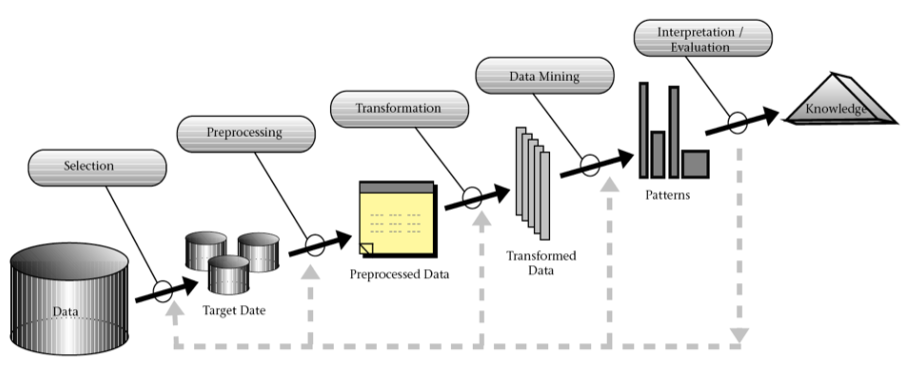
\includegraphics[width=\textwidth]{images/DM_Process.png}










\chapter{Data Selection}
\label{cha:data_selection}
The selected dataset onto which a classification model shall be learned is provided by Kaggle \footnote{2017 Kaggle Inc}. It is named \textit{The movies Dataset}\footnote{Link to the dataset: \hyperref[https://www.kaggle.com/rounakbanik/the-movies-dataset]{https://www.kaggle.com/rounakbanik/the-movies-dataset}} and contains metadata on approximately 45,000 movies in its raw format. It is provided and updated by Rounik Banik. The csv-file has 24 columns.\\\\
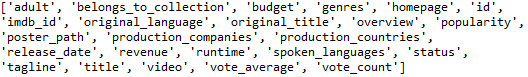
\includegraphics[width=\textwidth]{images/Raw_dataset_headers.png}
Untertitel bla bla


\textcolor{red}{\textit{unvollstaendige daten erlaeutern, grundlegende Graphen zeichnen lassen}}




\begin{itemize}
	\item In slides named: "structure and size of data"
	\item min. 1 Page
	\item Selection: 
	\begin{itemize}
		\item What data is available?
		\item What do I know about the provenance of the data?
		\item What do I know about the quality of the data?
	\end{itemize}
	\item Exploration
	\begin{itemize}
		\item Get an initial understanding of the data
		\item Calculate basic summarization statistics
		\item Visualize the data
		\item Identify data problems such as outliers, missing values, duplicate records
	\end{itemize}
\end{itemize}



\chapter{Preprocessing and Transformation}
\label{cha:preprocessing_transformation}

In order to pick out columns that have a significant impact on forecasting a movie's success, the following assumptions concerning the importance of information in the metadata were made:
\begin{itemize}
	\item The budget and revenue are crucial numbers.
	\item The release year has an impact on numbers such as budget and revenue.
	\item The genre, the production company and the runtime are important information.
\end{itemize}

\begin{itemize}
	\item Transform data into a representation that is suitable for the chosen data mining methods
	\begin{itemize}
		\item number of dimensions
		\item scales of attributes (nominal, ordinal, numeric)
		\item amount of data (determines hardware requirements)
	\end{itemize}
	\item Methods
	\begin{itemize}
		\item Aggregation, sampling
		\item Dimensionality reduction / feature subset selection
		\item Attribute transformation / text to term vector
		\item Discretization and binarization
	\end{itemize}
	\item Good data preparation is key to producing valid and reliable models
	\item Data preparation estimated to take 70-80\% of the time and effort of a data mining project!
\end{itemize}

\section{A list of problems we encountered}
\begin{enumerate}
	\item \textbf{list further problems we had and solved!}
	\item Prod. Comp.: Same prod. company named differently -> using Regex to solve (Steffen)
	\item dataset: 5 datasets have duplicates
\end{enumerate}



\chapter{Data Mining}
\label{cha:data_mining}
\begin{itemize}
	\item Input: Preprocessed Data
	\item Output: Model / Patterns
\end{itemize}

\begin{enumerate}
	\item Apply data mining method
	\item Evaluate resulting model / patterns (using P, R, F1, not accuracy)
	\item Iterate:
	\begin{itemize}
		\item Experiment with different parameter settings
		\item Experiment with different alternative methods – Improve preprocessing and feature generation – Combine different methods
	\end{itemize}
\end{enumerate}

\section{Algorithms}



\chapter{Interpretation / Evaluation}
\label{cha:interpretation_evaluation}
Maybe also prospect?
\begin{itemize}
	\item Output of Data Mining
	\begin{itemize}
		\item Patterns
		\item Models
	\end{itemize}
	\item In the end, we want to derive value from that, e.g.,
	\begin{itemize}
		\item gain knowledge
		\item make better decisions
		\item increase revenue
	\end{itemize}
\end{itemize}



